\chapter{多变量函数的微分学}


\section{多变量函数及其连续性}

\begin{problem}{德·摩根定律}{De-Morgan-Laws}
    证明：$(A \cap B)^c = A^c \cup B^c$ 且 $(A \cup B)^c = A^c \cap B^c$。
\end{problem}

\begin{myproof}
    根据集合相等的定义，通过证明元素的等价性来完成推导。对于第一个等式：
    \begin{equation*}
        \begin{aligned}
            x \in (A \cap B)^c & \iff x \notin A \cap B              \\
                               & \iff \neg (x \in A \land x \in B)   \\
                               & \iff (x \notin A) \lor (x \notin B) \\
                               & \iff (x \in A^c) \lor (x \in B^c)   \\
                               & \iff x \in A^c \cup B^c
        \end{aligned}
    \end{equation*}
    从而得证：
    \begin{equation*}
        \boxed{(A \cap B)^c = A^c \cup B^c}
    \end{equation*}
    对于第二个等式，同理可得：
    \begin{equation*}
        \begin{aligned}
            x \in (A \cup B)^c & \iff x \notin A \cup B               \\
                               & \iff \neg (x \in A \lor x \in B)     \\
                               & \iff (x \notin A) \land (x \notin B) \\
                               & \iff (x \in A^c) \land (x \in B^c)   \\
                               & \iff x \in A^c \cap B^c
        \end{aligned}
    \end{equation*}
    从而得证：
    \begin{equation*}
        \boxed{(A \cup B)^c = A^c \cap B^c}
    \end{equation*}
\end{myproof}


\begin{problem}{开集与闭集的运算性质}{Open-Closed-Sets-Operations}
    证明两个开集的交集和并集仍是开集，两个闭集的交集和并集仍是闭集。
\end{problem}

\begin{myproof}
    设 $G_1, G_2$ 为两个开集。
    \begin{itemize}
        \item 对于并集 $G_1 \cup G_2$：任取 $x \in G_1 \cup G_2$，则 $x \in G_1$ 或 $x \in G_2$。不妨设 $x \in G_1$，由 $G_1$ 的开性知，$\exists \delta > 0$ 使得 $B(x, \delta) \subset G_1 \subset G_1 \cup G_2$，故 $G_1 \cup G_2$ 为开集。
        \item 对于交集 $G_1 \cap G_2$：任取 $x \in G_1 \cap G_2$，则 $x \in G_1$ 且 $x \in G_2$。由 $G_1, G_2$ 的开性知：
              \begin{equation*}
                  \exists \delta_1 > 0, B(x, \delta_1) \subset G_1 \quad \text{且} \quad \exists \delta_2 > 0, B(x, \delta_2) \subset G_2
              \end{equation*}
              令 $\delta = \min\{\delta_1, \delta_2\} > 0$，则 $B(x, \delta) \subset G_1 \cap G_2$，故 $G_1 \cap G_2$ 为开集。
    \end{itemize}
    设 $F_1, F_2$ 为两个闭集，则其补集 $F_1^c, F_2^c$ 为开集。由德·摩根定律：
    \begin{equation*}
        (F_1 \cup F_2)^c = F_1^c \cap F_2^c, \quad (F_1 \cap F_2)^c = F_1^c \cup F_2^c
    \end{equation*}
    由于开集的有限交与有限并仍为开集，可知 $(F_1 \cup F_2)^c$ 与 $(F_1 \cap F_2)^c$ 均为开集。根据闭集定义，其补集 $F_1 \cup F_2$ 与 $F_1 \cap F_2$ 均为闭集。综上所述：
    \begin{equation*}
        \boxed{\text{两个开集的交、并集仍为开集；两个闭集的交、并集仍为闭集}}
    \end{equation*}
\end{myproof}


\begin{problem}{开集与边界}{Open-Set-Boundary}
    证明：满足 $y > ax + b$ 的所有点 $(x, y)$ 是一个开集。在坐标平面上画出它的范围，并求它的边界点应满足的关系。
\end{problem}

\begin{myproof}
    令 $f(x, y) = y - ax - b$，则 $f: \symbb{R}^2 \to \symbb{R}$ 为连续函数。
    设集合 $S = \{ (x, y) \in \symbb{R}^2 \mid y > ax + b \}$，则有
    \begin{equation*}
        S = \{ (x, y) \in \symbb{R}^2 \mid f(x, y) \in (0, +\infty) \} = f^{-1}\bigl( (0, +\infty) \bigr)
    \end{equation*}
    由于 $(0, +\infty)$ 是 $\symbb{R}$ 中的开集，且连续函数的原像是开集，故 $S$ 是 $\symbb{R}^2$ 中的一个开集。

    其范围在坐标平面上的示意图如下（以 $a > 0, b > 0$ 为例）：
    \begin{center}
        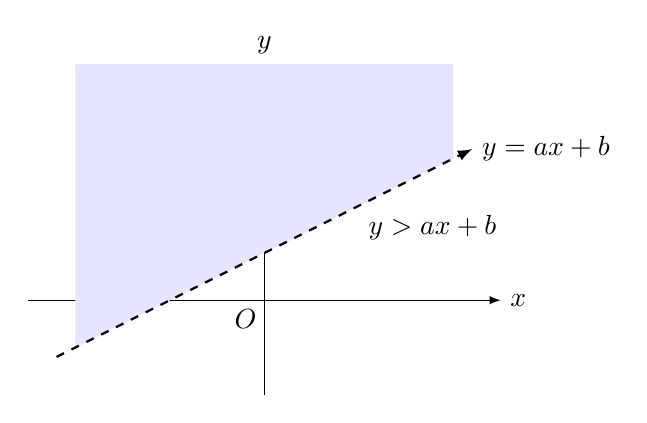
\begin{tikzpicture}[-latex, scale=1.2]
            \draw (-2.5, 0) -- (2.5, 0) node[right] {$x$};
            \draw (0, -1) -- (0, 2.5) node[above] {$y$};
            \node at (-0.2, -0.2) {$O$};
            \fill[blue!10] (-2, -0.5) -- (2, 1.5) -- (2, 2.5) -- (-2, 2.5) -- cycle;
            \draw[dashed, thick, domain=-2.2:2.2] plot (\x, {0.5*\x + 0.5});
            \node[below right] at (1, 1) {$y > ax + b$};
            \node[right] at (2.2, 1.6) {$y = ax + b$};
        \end{tikzpicture}
    \end{center}

    该集合的闭包为 $\overline{S} = \{ (x, y) \mid y \ge ax + b \}$，其内部为 $S^\circ = S$。
    根据边界的定义 $\partial S = \overline{S} \setminus S^\circ$，可得边界点应满足的关系为
    \begin{equation*}
        \boxed{y = ax + b}
    \end{equation*}
\end{myproof}


\begin{problem}{距离函数的连续性}{Distance-Function-Continuity}
    设 $\lim M_n = M_0, \lim M'_n = M'_0$. 求证: $\lim \rho(M_n, M'_n) = \rho(M_0, M'_0)$.
\end{problem}

\begin{myproof}
    根据度量空间的三角不等式，有
    \begin{equation*}
        \rho(M_n, M'_n) \le \rho(M_n, M_0) + \rho(M_0, M'_0) + \rho(M'_0, M'_n)
    \end{equation*}
    由此可得
    \begin{equation*}
        \rho(M_n, M'_n) - \rho(M_0, M'_0) \le \rho(M_n, M_0) + \rho(M'_n, M'_0)
    \end{equation*}
    同理，交换位置可得
    \begin{equation*}
        \rho(M_0, M'_0) \le \rho(M_0, M_n) + \rho(M_n, M'_n) + \rho(M'_n, M'_0)
    \end{equation*}
    从而有
    \begin{equation*}
        \rho(M_0, M'_0) - \rho(M_n, M'_n) \le \rho(M_n, M_0) + \rho(M'_n, M'_0)
    \end{equation*}
    综合上述两个不等式，得到
    \begin{equation*}
        |\rho(M_n, M'_n) - \rho(M_0, M'_0)| \le \rho(M_n, M_0) + \rho(M'_n, M'_0)
    \end{equation*}
    由于已知 $\lim M_n = M_0$ 且 $\lim M'_n = M'_0$, 即
    \begin{equation*}
        \lim_{n \to \infty} \rho(M_n, M_0) = 0, \quad \lim_{n \to \infty} \rho(M'_n, M'_0) = 0
    \end{equation*}
    由夹逼定理可知
    \begin{equation*}
        \lim_{n \to \infty} |\rho(M_n, M'_n) - \rho(M_0, M'_0)| = 0
    \end{equation*}
    故命题得证
    \begin{equation*}
        \lim_{n \to \infty} \rho(M_n, M'_n) = \rho(M_0, M'_0)
    \end{equation*}
\end{myproof}


\begin{problem}{收敛点列的有界性}{Convergence-Boundedness}
    证明：平面上收敛的点列必然是有界的.
\end{problem}

\begin{myproof}
    设平面点列 $\{P_n\}$ 收敛于 $P_0$.
    根据收敛定义，取 $\varepsilon = 1$, 必存在正整数 $N$, 使得当 $n > N$ 时, 恒有
    \begin{equation*}
        \rho(P_n, P_0) < 1
    \end{equation*}
    令
    \begin{equation*}
        R = \max \left\{ \rho(P_1, P_0), \rho(P_2, P_0), \dots, \rho(P_N, P_0), 1 \right\}
    \end{equation*}
    显然 $R > 0$. 对于任意正整数 $n$:
    \begin{enumerate}
        \item 若 $n \le N$, 则 $\rho(P_n, P_0) \le \max \{ \rho(P_1, P_0), \dots, \rho(P_N, P_0) \} \le R$;
        \item 若 $n > N$, 则 $\rho(P_n, P_0) < 1 \le R$.
    \end{enumerate}
    综上所述, 对于所有正整数 $n$, 恒有 $\rho(P_n, P_0) \le R$.
    这说明点列 $\{P_n\}$ 包含在以 $P_0$ 为圆心, $R$ 为半径的闭圆盘内, 因此该点列是有界的.
\end{myproof}


\begin{problem}{拓扑正弦曲线}{Topologists-Sine-Curve}
    证明集合 $E = \{(x,y) : y = \sin \frac{1}{x}, 0 < x \leqslant \frac{2}{\uppi}\} \cup \{(0,y) : 0 \leqslant y \leqslant 1\}$ 是连通的但不是道路连通的。

    \begin{center}
        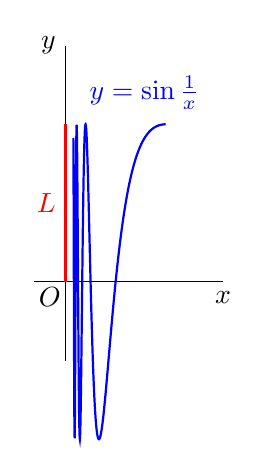
\begin{tikzpicture}[scale=2, >=latex]
            \draw (0,-0.5) -- (0,1.5) node[left] {$y$};
            \draw (-0.2,0) -- (1,0) node[below] {$x$};
            \node at (-0.1,-0.1) {$O$};
            \draw[thick, blue, domain=0.05:0.6366, samples=500] plot (\x, {sin(1/\x r)});
            \draw[thick, red] (0,0) -- (0,1);
            \node[blue] at (0.5,1.2) {$y = \sin \frac{1}{x}$};
            \node[red, left] at (0,0.5) {$L$};
        \end{tikzpicture}
    \end{center}
\end{problem}

\begin{myproof}
    令 $E_1 = \left\{ \left(x, \sin \frac{1}{x}\right) : 0 < x \leqslant \frac{2}{\uppi} \right\}$ 且 $L = \{(0, y) : 0 \leqslant y \leqslant 1\}$，则 $E = E_1 \cup L$。

    1. \textbf{连通性证明}：
    由于 $E_1$ 是连续函数 $f(x) = \sin \frac{1}{x}$ 在连通集 $(0, 2/\uppi]$ 上的图像，故 $E_1$ 是道路连通的，从而也是连通的。
    对于任意 $y \in [0, 1]$，取序列 $x_n = \left( 2n\uppi + \arcsin y \right)^{-1}$，当 $n \to \infty$ 时，$x_n \to 0^+$ 且 $\sin(1/x_n) = y$。
    这意味着 $(x_n, y) \in E_1$ 且 $(x_n, y) \to (0, y)$，故 $L \subset \overline{E_1}$。
    根据连通集的性质，若 $E_1 \subset E \subset \overline{E_1}$ 且 $E_1$ 连通，则 $E$ 必为连通集。

    2. \textbf{非道路连通性证明}：
    假设 $E$ 是道路连通的，则存在连续映射 $\symbfit{\gamma}(t) = (x(t), y(t))$，其中 $t \in [0, 1]$，使得 $\symbfit{\gamma}(0) = (0, 0) \in L$ 且 $\symbfit{\gamma}(1) = (2/\uppi, 1) \in E_1$。
    定义 $t_0 = \sup \{ t \in [0, 1] : x(t) = 0 \}$。由 $x(t)$ 的连续性及 $x(1) > 0$ 知 $0 \leqslant t_0 < 1$ 且 $x(t_0) = 0$。
    由于 $\symbfit{\gamma}(t) \in E$ 且对于 $t \in (t_0, 1]$ 有 $x(t) > 0$，故当 $t > t_0$ 时必有 $y(t) = \sin \frac{1}{x(t)}$。
    由 $\symbfit{\gamma}$ 在 $t_0$ 处的连续性可知：
    \begin{equation*}
        \lim_{t \to t_0^+} y(t) = y(t_0) \in [0, 1]
    \end{equation*}
    然而，由于 $\lim_{t \to t_0^+} x(t) = 0$，我们可以构造序列 $t_n \to t_0^+$ 使得 $x(t_n) = \frac{1}{2n\uppi - \uppi/2}$。此时：
    \begin{equation*}
        y(t_n) = \sin\left( 2n\uppi - \frac{\uppi}{2} \right) = -1
    \end{equation*}
    从而有 $\lim_{n \to \infty} y(t_n) = -1$，这要求 $y(t_0) = -1$。
    但这与 $y(t_0) \in [0, 1]$ 矛盾。故不存在这样的连续路径。

    \begin{equation*}
        \boxed{E \text{ 是连通的但不是道路连通的}}
    \end{equation*}
\end{myproof}


\begin{problem}{多元函数定义域与拓扑性质}{Domain-Topology}
    确定并画出以下函数的定义域, 并指出它们是否是区域, 是否是闭区域.
    \begin{enumerate}
        \item $z = \sqrt{x+y}$
        \item $z = \sqrt{x - 2y^2}$
        \item $z = \frac{\sqrt{x^2+y^2+2x}}{\sqrt{2x-x^2-y^2}}$
        \item $z = \sqrt{\sin(x^2+y^2)}$
        \item $z = \ln\left(1 - \frac{x^2}{a^2} - \frac{y^2}{b^2}\right)$
        \item $z = \sqrt{\cos x \sin y}$
        \item $u = \arcsin \frac{\sqrt{x^2+y^2}}{z}$
        \item $u = \sqrt{2az - x^2 - y^2 - z^2} \quad (a > 0)$
    \end{enumerate}
\end{problem}

\begin{solution}
    \ansitem{1}

    由 $x+y \ge 0 \implies y \ge -x$.
    \begin{center}
        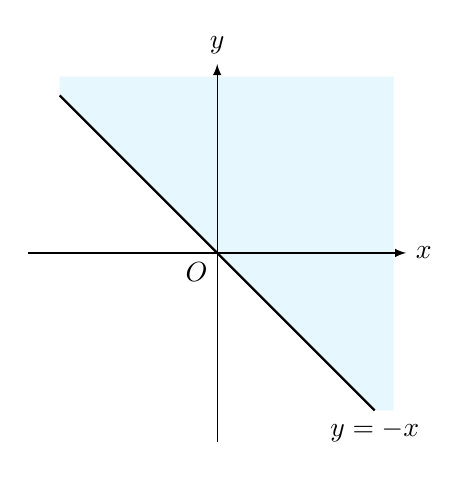
\begin{tikzpicture}[>=latex, scale=0.8]
            \fill[cyan!10] (-2.5,2.5) -- (2.5,-2.5) -- (2.8,-2.5) -- (2.8,2.8) -- (-2.5,2.8) -- cycle;
            \draw[->] (-3,0) -- (3,0) node[right] {$x$};
            \draw[->] (0,-3) -- (0,3) node[above] {$y$};
            \draw[thick, domain=-2.5:2.5] plot (\x, {-\x}) node[below] {$y=-x$};
            \node at (0,0) [below left] {$O$};
        \end{tikzpicture}
    \end{center}
    该集合是连通的闭集, 故其不是区域 (非开集), 是闭区域.
    \begin{equation*}
        \boxed{D = \{ (x, y) \mid x+y \ge 0 \}}
    \end{equation*}

    \ansitem{2}

    由 $x - 2y^2 \ge 0 \implies x \ge 2y^2$.
    \begin{center}
        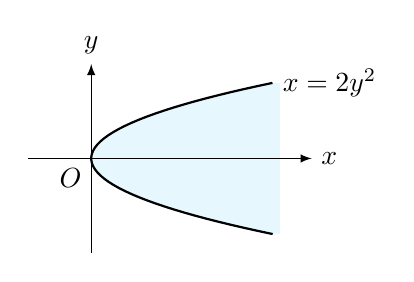
\begin{tikzpicture}[>=latex, scale=0.8]
            \fill[cyan!10, samples=50, domain=-1.2:1.2] plot ({2*\x*\x}, \x) -- (3, 1.2) -- (3, -1.2) -- cycle;
            \draw[->] (-1,0) -- (3.5,0) node[right] {$x$};
            \draw[->] (0,-1.5) -- (0,1.5) node[above] {$y$};
            \draw[thick, samples=50, domain=-1.2:1.2] plot ({2*\x*\x}, \x) node[right] {$x=2y^2$};
            \node at (0,0) [below left] {$O$};
        \end{tikzpicture}
    \end{center}
    该集合是连通的闭集, 故其不是区域, 是闭区域.
    \begin{equation*}
        \boxed{D = \{ (x, y) \mid x \ge 2y^2 \}}
    \end{equation*}

    \ansitem{3}

    需满足 $x^2+y^2+2x \ge 0$ 且 $2x-x^2-y^2 > 0$, 即:
    \begin{equation*}
        \begin{cases} (x+1)^2+y^2 \ge 1 \\ (x-1)^2+y^2 < 1 \end{cases}
    \end{equation*}
    由于圆盘 $(x-1)^2+y^2 < 1$ 除原点外均在 $(x+1)^2+y^2 > 1$ 范围内.
    \begin{center}
        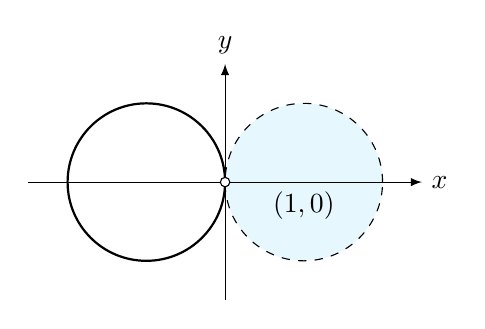
\begin{tikzpicture}[>=latex, scale=1]
            \draw[dashed, fill=cyan!10] (1,0) circle (1);
            \draw[thick] (-1,0) circle (1);
            \draw[->] (-2.5,0) -- (2.5,0) node[right] {$x$};
            \draw[->] (0,-1.5) -- (0,1.5) node[above] {$y$};
            \fill[white] (0,0) circle (0.06);
            \draw (0,0) circle (0.06);
            \node at (1,0) [below] {$(1,0)$};
        \end{tikzpicture}
    \end{center}
    该集合是连通开集, 故其是区域, 不是闭区域.
    \begin{equation*}
        \boxed{D = \{ (x, y) \mid (x-1)^2+y^2 < 1, (x, y) \neq (0,0) \}}
    \end{equation*}

    \ansitem{4}

    由 $\sin(x^2+y^2) \ge 0 \implies 2k\uppi \le x^2+y^2 \le (2k+1)\uppi \quad (k = 0, 1, 2, \dots)$.
    \begin{center}
        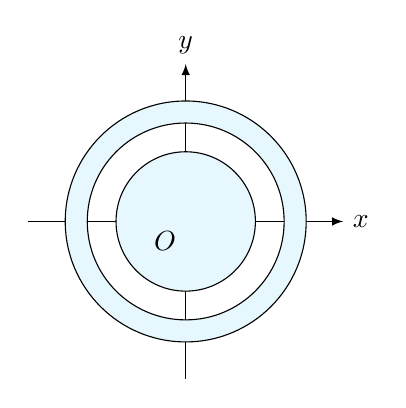
\begin{tikzpicture}[>=latex, scale=0.5]
            \draw[->] (-4,0) -- (4,0) node[right] {$x$};
            \draw[->] (0,-4) -- (0,4) node[above] {$y$};
            \fill[cyan!10, even odd rule] (0,0) circle (1.77) (0,0) circle (0);
            \fill[cyan!10, even odd rule] (0,0) circle (3.06) (0,0) circle (2.5);
            \draw (0,0) circle (1.77); \draw (0,0) circle (2.5); \draw (0,0) circle (3.06);
            \node at (0,0) [below left] {$O$};
        \end{tikzpicture}
    \end{center}
    该集合由互不相连的闭环带组成, 不连通, 故既不是区域, 也不是闭区域.
    \begin{equation*}
        \boxed{D = \bigcup_{k=0}^{\infty} \{ (x, y) \mid 2k\uppi \le x^2+y^2 \le (2k+1)\uppi \}}
    \end{equation*}

    \ansitem{5}

    由 $1 - \frac{x^2}{a^2} - \frac{y^2}{b^2} > 0 \implies \frac{x^2}{a^2} + \frac{y^2}{b^2} < 1$.
    \begin{center}
        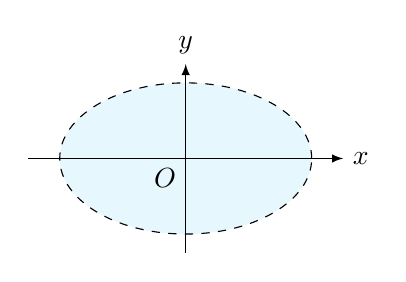
\begin{tikzpicture}[>=latex, scale=0.8]
            \draw[dashed, fill=cyan!10] (0,0) ellipse (2 and 1.2);
            \draw[->] (-2.5,0) -- (2.5,0) node[right] {$x$};
            \draw[->] (0,-1.5) -- (0,1.5) node[above] {$y$};
            \node at (0,0) [below left] {$O$};
        \end{tikzpicture}
    \end{center}
    此为椭圆内部开集, 且连通, 故其是区域, 不是闭区域.
    \begin{equation*}
        \boxed{D = \left\{ (x, y) \mid \frac{x^2}{a^2} + \frac{y^2}{b^2} < 1 \right\}}
    \end{equation*}

    \ansitem{6}

    由 $\cos x \sin y \ge 0$.
    \begin{center}
        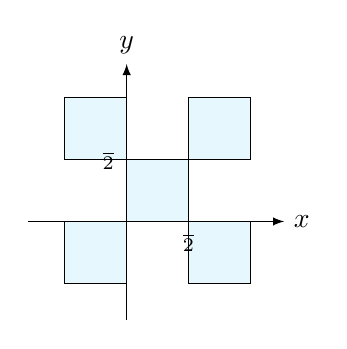
\begin{tikzpicture}[>=latex, scale=0.5]
            \foreach \i in {-1, 0, 1} \foreach \j in {-1, 0, 1} {
                    \pgfmathparse{mod(\i+\j, 2) == 0 ? 1 : 0}
                    \ifnum\pgfmathresult=1
                        \fill[cyan!10] ({\i*1.57}, {\j*1.57}) rectangle ({(\i+1)*1.57}, {(\j+1)*1.57});
                        \draw ({\i*1.57}, {\j*1.57}) rectangle ({(\i+1)*1.57}, {(\j+1)*1.57});
                    \fi
                }
            \draw[->] (-2.5,0) -- (4,0) node[right] {$x$};
            \draw[->] (0,-2.5) -- (0,4) node[above] {$y$};
            \node at (1.57,0) [below] {$\frac{\uppi}{2}$};
            \node at (0,1.57) [left] {$\frac{\uppi}{2}$};
        \end{tikzpicture}
    \end{center}
    该集合由离散分布的闭矩形块组成, 不连通, 故既不是区域, 也不是闭区域.
    \begin{equation*}
        \boxed{D = \{ (x, y) \mid \cos x \sin y \ge 0 \}}
    \end{equation*}

    \ansitem{7}

    需满足 $\left| \frac{\sqrt{x^2+y^2}}{z} \right| \le 1$ 且 $z \neq 0$, 即 $x^2+y^2 \le z^2$ 且 $z \neq 0$.
    \begin{center}
        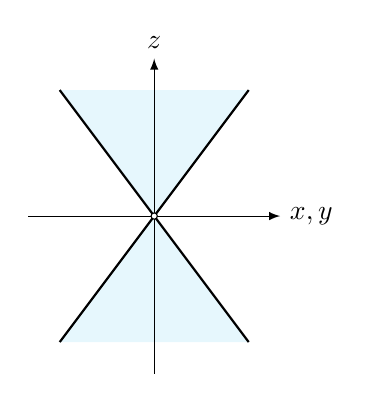
\begin{tikzpicture}[>=latex, scale=0.8]
            \fill[cyan!10] (0,0) -- (1.5,2) -- (-1.5,2) -- cycle;
            \fill[cyan!10] (0,0) -- (1.5,-2) -- (-1.5,-2) -- cycle;
            \draw[thick] (-1.5,2) -- (1.5,-2);
            \draw[thick] (1.5,2) -- (-1.5,-2);
            \draw[->] (-2,0) -- (2,0) node[right] {$x,y$};
            \draw[->] (0,-2.5) -- (0,2.5) node[above] {$z$};
            \fill[white] (0,0) circle (0.05);
            \draw (0,0) circle (0.05);
        \end{tikzpicture}
    \end{center}
    该集合在原点处断开, 不连通, 故既不是区域, 也不是闭区域.
    \begin{equation*}
        \boxed{D = \{ (x, y, z) \mid x^2+y^2 \le z^2, z \neq 0 \}}
    \end{equation*}

    \ansitem{8}

    由 $2az - x^2 - y^2 - z^2 \ge 0 \implies x^2 + y^2 + (z-a)^2 \le a^2$.
    \begin{center}
        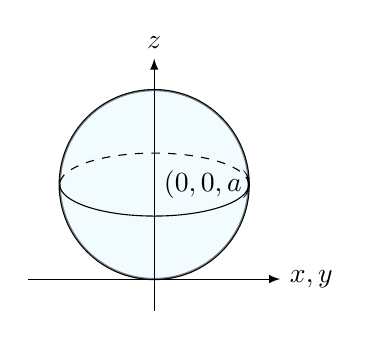
\begin{tikzpicture}[>=latex, scale=0.8]
            \draw[thick] (0,1.5) circle (1.5);
            \fill[cyan!10, opacity=0.5] (0,1.5) circle (1.5);
            \draw[dashed] (1.5,1.5) arc (0:180:1.5 and 0.5);
            \draw (1.5,1.5) arc (0:-180:1.5 and 0.5);
            \draw[->] (-2,0) -- (2,0) node[right] {$x,y$};
            \draw[->] (0,-0.5) -- (0,3.5) node[above] {$z$};
            \node at (0,1.5) [right] {$(0,0,a)$};
        \end{tikzpicture}
    \end{center}
    该集合是连通的闭球体, 故其不是区域, 是闭区域.
    \begin{equation*}
        \boxed{D = \{ (x, y, z) \mid x^2 + y^2 + (z-a)^2 \le a^2 \}}
    \end{equation*}
\end{solution}


\begin{problem}{多元函数图形与等高线}{Surface-Level-Curves}
    画出函数 $z = \cos(2x + y)$ 的略图以及对应于 $z = 0, \pm 1, \pm \frac{1}{2}$ 的等高线。
\end{problem}

\begin{solution}
    \ansitem{1}
    函数 $z = \cos(2x + y)$ 的图形是一个沿直线 $2x + y = C$ 方向延伸的波浪状柱面。其在 $xy$ 平面上的截痕为一系列平行的直线，数值随垂直于这些直线的方向呈余弦规律波动。

    \begin{center}
        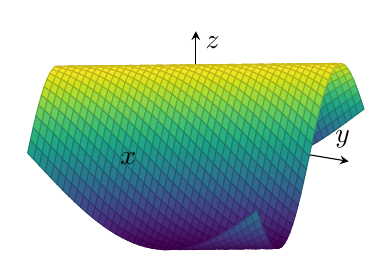
\begin{tikzpicture}
            \begin{axis}[
                    width=0.6\textwidth,
                    view={115}{30},
                    axis lines=center,
                    xlabel=$x$, ylabel=$y$, zlabel=$z$,
                    xmin=-2, xmax=2, ymin=-2, ymax=2, zmin=-1.5, zmax=1.5,
                    ticks=none,
                    colormap/viridis
                ]
                \addplot3[surf, domain=-1.5:1.5, y domain=-1.5:1.5, samples=40] {cos(deg(2*x + y))};
            \end{axis}
        \end{tikzpicture}
    \end{center}

    \ansitem{2}
    令 $z = C$（其中 $C \in [-1, 1]$），则等高线方程为 $\cos(2x + y) = C$。由此得：
    \begin{equation*}
        2x + y = 2k\uppi \pm \arccos C, \quad k \in \symbb{Z}
    \end{equation*}
    这是一组斜率为 $-2$ 的平行直线族。针对给定的 $z$ 值，等高线方程如下：
    \begin{equation*}
        \begin{aligned}
            z = 1            & \implies 2x + y = 2k\uppi                         \\
            z = -1           & \implies 2x + y = (2k+1)\uppi                     \\
            z = 0            & \implies 2x + y = k\uppi + \frac{\uppi}{2}        \\
            z = \frac{1}{2}  & \implies 2x + y = 2k\uppi \pm \frac{\uppi}{3}     \\
            z = -\frac{1}{2} & \implies 2x + y = (2k+1)\uppi \pm \frac{\uppi}{3}
        \end{aligned}
    \end{equation*}

    \begin{center}
        \begin{tikzpicture}[scale=0.8]
            \draw[-latex] (-3,0) -- (3,0) node[right] {$x$};
            \draw[-latex] (0,-4) -- (0,4) node[above] {$y$};
            \node at (0.2,-0.2) {$O$};
            \clip (-2.5,-3.5) rectangle (2.5,3.5);
            % z=1 (solid red)
            \draw[red, thick] plot[domain=-2:2] (\x, {-2*\x});
            \draw[red, thick] plot[domain=-2:2] (\x, {-2*\x + 6.28});
            \draw[red, thick] plot[domain=-2:2] (\x, {-2*\x - 6.28});
            % z=0 (dashed blue)
            \draw[blue, dashed] plot[domain=-2:2] (\x, {-2*\x + 1.57});
            \draw[blue, dashed] plot[domain=-2:2] (\x, {-2*\x - 1.57});
            % z=-1 (dotted black)
            \draw[black, dash dot] plot[domain=-2:2] (\x, {-2*\x + 3.14});
            \draw[black, dash dot] plot[domain=-2:2] (\x, {-2*\x - 3.14});
        \end{tikzpicture}
    \end{center}
    综上所述，该函数的等高线方程为：
    \begin{equation*}
        \boxed{y = -2x + 2k\uppi \pm \arccos z, \quad k \in \symbb{Z}}
    \end{equation*}
\end{solution}


\begin{problem}{多项式项数}{Polynomial-Terms}
    一个变量的一般形式的 $n$ 次多项式共有 $n+1$ 项单项式 $x^0, x^1, \dots, x^n$。如果对于两个变量而言，单项式定义为 $x^k y^l$，次数定义为 $k+l$，问一般形式的 $n$ 次二元多项式共有多少项单项式？
\end{problem}

\begin{solution}
    设二元单项式为 $x^k y^l$，其次数为 $k+l = m$。对于固定的次数 $m \in \{0, 1, \dots, n\}$，满足要求的非负整数对 $(k, l)$ 的个数即为该次数下的单项式数，共有 $m+1$ 个。

    一般形式的 $n$ 次二元多项式包含所有次数满足 $0 \le m \le n$ 的项。记总项数为 $N$，则有：
    \begin{equation*}
        \begin{aligned}
            N & = \sum_{m=0}^{n} (m+1)         \\
              & = 1 + 2 + \cdots + (n+1)       \\
              & = \frac{(1 + n + 1)(n + 1)}{2} \\
              & = \frac{(n+1)(n+2)}{2}
        \end{aligned}
    \end{equation*}

    由此得到最终结果：
    \begin{equation*}
        \boxed{N = \frac{(n+1)(n+2)}{2}}
    \end{equation*}
\end{solution}


\begin{problem}{多元函数求值}{Multivariable-Function-Evaluation}
    设 $f(x, y) = \frac{2xy}{x^2+y^2}$，求 $f(1, 1), f(y, x), f(1, \frac{y}{x}), f(u, v), f(\cos t, \sin t)$。
\end{problem}

\begin{solution}
    直接代入定义式计算：
    \begin{equation*}
        \begin{aligned}
            f(1, 1)                        & = \frac{2 \cdot 1 \cdot 1}{1^2 + 1^2} = 1                                                                                                     \\
            f(y, x)                        & = \frac{2yx}{y^2 + x^2} = \frac{2xy}{x^2 + y^2}                                                                                               \\
            f\left( 1, \frac{y}{x} \right) & = \frac{2 \cdot 1 \cdot \frac{y}{x}}{1^2 + \left( \frac{y}{x} \right)^2} = \frac{\frac{2y}{x}}{\frac{x^2 + y^2}{x^2}} = \frac{2xy}{x^2 + y^2} \\
            f(u, v)                        & = \frac{2uv}{u^2 + v^2}                                                                                                                       \\
            f(\cos t, \sin t)              & = \frac{2\cos t \sin t}{\cos^2 t + \sin^2 t} = \frac{\sin 2t}{1} = \sin 2t
        \end{aligned}
    \end{equation*}
    综上所述，结果分别为：
    \begin{equation*}
        \boxed{f(1, 1) = 1, f(y, x) = \frac{2xy}{x^2+y^2}, f\left( 1, \frac{y}{x} \right) = \frac{2xy}{x^2+y^2}, f(u, v) = \frac{2uv}{u^2+v^2}, f(\cos t, \sin t) = \sin 2t}
    \end{equation*}
\end{solution}

\begin{problem}{复合函数解析式}{Composite-Function}
    设 $f(x, y) = \begin{cases} 1, & y \geqslant x, \\ 0, & y < x, \end{cases}$ 又 $\begin{cases} x = \cos t, \\ y = \sin t, \end{cases}$ 求 $F(t) = f(\cos t, \sin t)$。
\end{problem}

\begin{solution}
    根据定义 $F(t) = f(\cos t, \sin t)$，需比较 $\sin t$ 与 $\cos t$ 的大小关系：
    \begin{equation*}
        \sin t \geqslant \cos t \iff \sqrt{2}\sin\left( t - \frac{\uppi}{4} \right) \geqslant 0 \iff 2k\uppi + \frac{\uppi}{4} \leqslant t \leqslant 2k\uppi + \frac{5\uppi}{4}, \quad k \in \symbb{Z}
    \end{equation*}
    因此，函数 $F(t)$ 的表达式为：
    \begin{equation*}
        \boxed{F(t) = \begin{cases} 1, & 2k\uppi + \frac{\uppi}{4} \leqslant t \leqslant 2k\uppi + \frac{5\uppi}{4} \\ 0, & 2k\uppi - \frac{3\uppi}{4} < t < 2k\uppi + \frac{\uppi}{4} \end{cases} \quad (k \in \symbb{Z})}
    \end{equation*}
\end{solution}

\begin{problem}{抽象函数求值与表达式}{Function-Expression}
    设 $f(x + y, \frac{y}{x}) = x^2 - y^2 \ (x \neq 0)$，求 $f(2, 3), f(x, y)$。
\end{problem}

\begin{solution}
    \ansitem{1}
    令 $x + y = 2$ 且 $\frac{y}{x} = 3$，由后者得 $y = 3x$。代入前者：
    \begin{equation*}
        x + 3x = 2 \implies 4x = 2 \implies x = \frac{1}{2}, \quad y = \frac{3}{2}
    \end{equation*}
    代入原函数关系式得：
    \begin{equation*}
        f(2, 3) = \left( \frac{1}{2} \right)^2 - \left( \frac{3}{2} \right)^2 = \frac{1}{4} - \frac{9}{4} = -2
    \end{equation*}
    \begin{equation*}
        \boxed{f(2, 3) = -2}
    \end{equation*}

    \ansitem{2}
    设 $u = x + y, v = \frac{y}{x}$，则 $y = vx$。代入 $u$ 的表达式：
    \begin{equation*}
        x + vx = u \implies x = \frac{u}{1+v}, \quad y = \frac{uv}{1+v}
    \end{equation*}
    将其代入 $f(u, v)$：
    \begin{equation*}
        \begin{aligned}
            f(u, v) & = \left( \frac{u}{1+v} \right)^2 - \left( \frac{uv}{1+v} \right)^2 \\
                    & = \frac{u^2(1 - v^2)}{(1+v)^2}                                     \\
                    & = \frac{u^2(1-v)(1+v)}{(1+v)^2}                                    \\
                    & = \frac{u^2(1-v)}{1+v}
        \end{aligned}
    \end{equation*}
    将变量名替换回 $x, y$ 得：
    \begin{equation*}
        \boxed{f(x, y) = \frac{x^2(1-y)}{1+y}}
    \end{equation*}
\end{solution}

\begin{problem}{多元复合函数}{Multivariable-Composition}
    设 $f(x, y) = x^y, \varphi(x, y) = x + y, \psi(x, y) = x - y$，求 $f[\varphi(x, y), \psi(x, y)], \varphi[f(x, y), \psi(x, y)], \psi[\varphi(x, y), f(x, y)]$。
\end{problem}

\begin{solution}
    依次进行复合代入：
    \begin{equation*}
        \begin{aligned}
            f[\varphi(x, y), \psi(x, y)] & = f(x+y, x-y) = (x+y)^{x-y}                     \\
            \varphi[f(x, y), \psi(x, y)] & = \varphi(x^y, x-y) = x^y + (x-y) = x^y + x - y \\
            \psi[\varphi(x, y), f(x, y)] & = \psi(x+y, x^y) = (x+y) - x^y = x + y - x^y
        \end{aligned}
    \end{equation*}
    最终结果为：
    \begin{equation*}
        \boxed{f[\varphi, \psi] = (x+y)^{x-y}, \quad \varphi[f, \psi] = x^y + x - y, \quad \psi[\varphi, f] = x + y - x^y}
    \end{equation*}
\end{solution}


\begin{problem}{多元函数极限}{Multivariable-Limit}
    判断下列各题极限是否存在，若有极限，求出其极限：
    \begin{enumerate}
        \item $\lim_{\substack{x \to 0 \\ y \to 0}} \frac{x^2 + y^2}{|x| + |y|}$
        \item $\lim_{\substack{x \to 0 \\ y \to a}} \frac{\sin xy}{x}$
        \item $\lim_{\substack{x \to +\infty \\ y \to +\infty}} \left( \frac{xy}{x^2 + y^2} \right)^{x^2}$
        \item $\lim_{\substack{x \to \infty \\ y \to a}} \left( 1 + \frac{1}{x} \right)^{\frac{x^2}{x+y}}$
        \item $\lim_{\substack{x \to 0 \\ y \to 0}} \frac{x^3 + y^3}{x^2 + y^2}$
        \item $\lim_{\substack{x \to \infty \\ y \to \infty}} \frac{x^2 + y^2}{x^4 + y^4}$
        \item $\lim_{\substack{x \to +\infty \\ y \to +\infty}} (x^2 + y^2) \e^{-(x+y)}$
        \item $\lim_{\substack{x \to 1 \\ y \to 0}} \frac{\ln (x + \e^y)}{\sqrt{x^2 + y^2}}$
        \item $\lim_{\substack{x \to 0 \\ y \to 0}} \frac{xy}{\sqrt{xy+1}-1}$
        \item $\lim_{\substack{x \to 0 \\ y \to 0}} \frac{\sqrt{xy+1}-1}{x+y}$
        \item $\lim_{\substack{x \to 0 \\ y \to 0}} \frac{1-\cos(x^2+y^2)}{(x^2+y^2)x^2y^2}$
        \item $\lim_{\substack{x \to 0 \\ y \to 0}} (1 + xy)^{\frac{1}{x+y}}$
    \end{enumerate}
\end{problem}

\begin{solution}
    \ansitem{1}
    因为 $0 \le \frac{x^2 + y^2}{|x| + |y|} \le \frac{x^2 + y^2 + 2|xy|}{|x| + |y|} = \frac{(|x| + |y|)^2}{|x| + |y|} = |x| + |y|$，
    又 $\lim_{\substack{x \to 0 \\ y \to 0}} (|x| + |y|) = 0$，由夹逼定理得：
    \begin{equation*}
        \boxed{\lim_{\substack{x \to 0 \\ y \to 0}} \frac{x^2 + y^2}{|x| + |y|} = 0}
    \end{equation*}

    \ansitem{2}
    当 $x \to 0, y \to a$ 时，$xy \to 0$，利用等价无穷小 $\sin xy \sim xy$ 得：
    \begin{equation*}
        \lim_{\substack{x \to 0 \\ y \to a}} \frac{\sin xy}{x} = \lim_{\substack{x \to 0 \\ y \to a}} \frac{xy}{x} = \lim_{y \to a} y = a
    \end{equation*}
    \begin{equation*}
        \boxed{\lim_{\substack{x \to 0 \\ y \to a}} \frac{\sin xy}{x} = a}
    \end{equation*}

    \ansitem{3}
    由于 $x^2 + y^2 \ge 2xy$，则 $0 < \frac{xy}{x^2 + y^2} \le \frac{1}{2}$，从而：
    \begin{equation*}
        0 < \left( \frac{xy}{x^2 + y^2} \right)^{x^2} \le \left( \frac{1}{2} \right)^{x^2}
    \end{equation*}
    由于 $\lim_{x \to +\infty} \left( \frac{1}{2} \right)^{x^2} = 0$，由夹逼定理知极限为 $0$。
    \begin{equation*}
        \boxed{\lim_{\substack{x \to +\infty \\ y \to +\infty}} \left( \frac{xy}{x^2 + y^2} \right)^{x^2} = 0}
    \end{equation*}

    \ansitem{4}
    利用重要极限 $\lim_{x \to \infty} (1 + 1/x)^x = \e$：
    \begin{equation*}
        \lim_{\substack{x \to \infty \\ y \to a}} \left( 1 + \frac{1}{x} \right)^{\frac{x^2}{x+y}} = \lim_{\substack{x \to \infty \\ y \to a}} \left[ \left( 1 + \frac{1}{x} \right)^x \right]^{\frac{x}{x+y}}
    \end{equation*}
    由 $\lim_{\substack{x \to \infty \\ y \to a}} \frac{x}{x+y} = \lim_{x \to \infty} \frac{1}{1 + a/x} = 1$，得：
    \begin{equation*}
        \boxed{\lim_{\substack{x \to \infty \\ y \to a}} \left( 1 + \frac{1}{x} \right)^{\frac{x^2}{x+y}} = \e}
    \end{equation*}

    \ansitem{5}
    采用极坐标变换，令 $x = r \cos \theta, y = r \sin \theta$：
    \begin{equation*}
        \left| \frac{x^3 + y^3}{x^2 + y^2} \right| = \left| \frac{r^3(\cos^3 \theta + \sin^3 \theta)}{r^2} \right| = r |\cos^3 \theta + \sin^3 \theta| \le 2r \to 0 \quad (r \to 0)
    \end{equation*}
    \begin{equation*}
        \boxed{\lim_{\substack{x \to 0 \\ y \to 0}} \frac{x^3 + y^3}{x^2 + y^2} = 0}
    \end{equation*}

    \ansitem{6}
    当 $x \to \infty, y \to \infty$ 时：
    \begin{equation*}
        0 \le \frac{x^2 + y^2}{x^4 + y^4} \le \frac{x^2}{x^4} + \frac{y^2}{y^4} = \frac{1}{x^2} + \frac{1}{y^2} \to 0
    \end{equation*}
    \begin{equation*}
        \boxed{\lim_{\substack{x \to \infty \\ y \to \infty}} \frac{x^2 + y^2}{x^4 + y^4} = 0}
    \end{equation*}

    \ansitem{7}
    由于 $(x^2 + y^2) \e^{-(x+y)} = \frac{x^2}{\e^x \e^y} + \frac{y^2}{\e^x \e^y}$，当 $x, y \to +\infty$ 时：
    \begin{equation*}
        \lim_{x \to +\infty} \frac{x^2}{\e^x} = 0, \quad \lim_{y \to +\infty} \frac{1}{\e^y} = 0 \implies \lim_{\substack{x \to +\infty \\ y \to +\infty}} \frac{x^2}{\e^{x+y}} = 0
    \end{equation*}
    同理 $\lim y^2 \e^{-(x+y)} = 0$，故：
    \begin{equation*}
        \boxed{\lim_{\substack{x \to +\infty \\ y \to +\infty}} (x^2 + y^2) \e^{-(x+y)} = 0}
    \end{equation*}

    \ansitem{8}
    函数在 $(1, 0)$ 处连续，直接代入得：
    \begin{equation*}
        \lim_{\substack{x \to 1 \\ y \to 0}} \frac{\ln (x + \e^y)}{\sqrt{x^2 + y^2}} = \frac{\ln(1 + \e^0)}{\sqrt{1^2 + 0^2}} = \frac{\ln 2}{1} = \ln 2
    \end{equation*}
    \begin{equation*}
        \boxed{\lim_{\substack{x \to 1 \\ y \to 0}} \frac{\ln (x + \e^y)}{\sqrt{x^2 + y^2}} = \ln 2}
    \end{equation*}

    \ansitem{9}
    利用分子有理化或等价无穷小 $\sqrt{u+1}-1 \sim \frac{1}{2}u$：
    \begin{equation*}
        \lim_{\substack{x \to 0 \\ y \to 0}} \frac{xy}{\sqrt{xy+1}-1} = \lim_{\substack{x \to 0 \\ y \to 0}} \frac{xy(\sqrt{xy+1}+1)}{(xy+1)-1} = \lim_{\substack{x \to 0 \\ y \to 0}} (\sqrt{xy+1}+1) = 2
    \end{equation*}
    \begin{equation*}
        \boxed{\lim_{\substack{x \to 0 \\ y \to 0}} \frac{xy}{\sqrt{xy+1}-1} = 2}
    \end{equation*}

    \ansitem{10}
    利用 $\sqrt{xy+1}-1 \sim \frac{1}{2}xy$。考查沿直线 $y = kx$ 趋于原点：
    \begin{equation*}
        \lim_{x \to 0} \frac{\frac{1}{2}kx^2}{(1+k)x} = \lim_{x \to 0} \frac{kx}{2(1+k)} = 0
    \end{equation*}
    再考查沿曲线 $y = -x + x^3$ 趋于原点：
    \begin{equation*}
        \lim_{x \to 0} \frac{\frac{1}{2}x(-x+x^3)}{x+(-x+x^3)} = \lim_{x \to 0} \frac{-\frac{1}{2}x^2 + \frac{1}{2}x^4}{x^3} = \lim_{x \to 0} \left( -\frac{1}{2x} + \frac{x}{2} \right) = \infty
    \end{equation*}
    由于趋近路径不同，极限值不同，故：
    \begin{equation*}
        \boxed{\text{该极限不存在}}
    \end{equation*}

    \ansitem{11}
    当 $x^2 + y^2 \to 0$ 时，$1 - \cos(x^2+y^2) \sim \frac{1}{2}(x^2+y^2)^2$：
    \begin{equation*}
        \lim_{\substack{x \to 0 \\ y \to 0}} \frac{1-\cos(x^2+y^2)}{(x^2+y^2)x^2y^2} = \lim_{\substack{x \to 0 \\ y \to 0}} \frac{\frac{1}{2}(x^2+y^2)^2}{(x^2+y^2)x^2y^2} = \lim_{\substack{x \to 0 \\ y \to 0}} \frac{x^2+y^2}{2x^2y^2} = \lim_{\substack{x \to 0 \\ y \to 0}} \left( \frac{1}{2y^2} + \frac{1}{2x^2} \right) = \infty
    \end{equation*}
    \begin{equation*}
        \boxed{\text{该极限不存在 (为 } \infty \text{)}}
    \end{equation*}

    \ansitem{12}
    令 $L = \lim_{\substack{x \to 0 \\ y \to 0}} (1 + xy)^{\frac{1}{x+y}}$，考虑其对数：
    \begin{equation*}
        \ln L = \lim_{\substack{x \to 0 \\ y \to 0}} \frac{\ln(1+xy)}{x+y} = \lim_{\substack{x \to 0 \\ y \to 0}} \frac{xy}{x+y}
    \end{equation*}
    在极坐标下：
    \begin{equation*}
        \left| \frac{xy}{x+y} \right| = \left| \frac{r^2 \cos \theta \sin \theta}{r(\cos \theta + \sin \theta)} \right| = r \left| \frac{\cos \theta \sin \theta}{\cos \theta + \sin \theta} \right|
    \end{equation*}
    在函数定义域内（需避开 $y=-x$），当 $r \to 0$ 时 $\ln L \to 0$，故 $L = \e^0 = 1$。
    \begin{equation*}
        \boxed{\lim_{\substack{x \to 0 \\ y \to 0}} (1 + xy)^{\frac{1}{x+y}} = 1}
    \end{equation*}
\end{solution}
